
\section{Desarrollo}


\subsection{Herramientas utilizadas en el proyecto}

Las herramientas utilizadas en este proyecto son QGIS, PostgreSQL y PostGIS.


\subsection{Datos}

Los datos utilizados en esta pŕactica corresponden a las trayectorias de
albatros de Laysan, registradas mediantes dispositivos GPS y GLS
\footnote{Sistema de posicionamiento global y sensor de localización global
respectivamente, por sus siglas en inglés}, de 47 individuos durante los años
2014 a 2018.

Los GPS se programaron para registrar simultáneamente la posición y la velocidad
del albatros cada 20 minutos, lo que permitió grabar de forma contínua durante
12 a 15 días en algunos casos y en otros de 60 a 70 días, durante la etapa
reproductiva \cite{hernandez2019ecologia}.

Para conocer los hábitos migratorios y zonas de distribución en temporada no
reproductiva se instalaron los dispositivos GLS, los cuales fueron recuperados
por lo menos un año después de su instalación.

Los datos crudos se encuentran en formato CSV y contienen los siguientes campos
o atributos:

\begin{table}[h!]
\caption{Campos o atributos de los datos crudos de trayectorias de albatros.}
\begin{center}
    \begin{tabular}{ l  m{7cm} }
        \hline
        Atributo & Descripción \\
        \hline
        date & Formato 'yyyy-mm-dd'. Se refiere a la fecha a la cual se registró
        la posición del ave. \\
        \hline
        latitude & Coordenada geográfica de la posición latitudinal del ave. \\
        \hline
        longitude & Coordenada geográfica de la posición longitudinal del ave.
        \\
        \hline
        name & Se refiere al id asociado al individuo de albatros de Laysan.\\
        \hline
    \end{tabular}
\end{center}
\end{table}

\subsection{Identificación del área de anidamiento de la especie}

El albatros de Laysan es una especie que presenta filopatría, esto quiere decir
que generalmente regresa a su colonia natal para reproducirse.

El albatros de Laysan se encuentra principalmente en el Pacífico Central (Islas
del noroeste de Hawai). Sin embargo en 1983, estableció una nueva colonia en
Isla Guadalupe.

Isla Guadalupe es una isla mexicana de origen volcánico, ubicada frente a la
costa de la península de Baja California y tiene una superficie total de
476,971. Está categorizada como Reserva de la Biosfera ha de acuerdo a la
Secretaría de Medio Ambiente y Recursos Naturales y a la Comisión Nacional de
Áreas Naturales Protegidas.

Isla Guadalupe se conforma de una isla principal y tres islotes principales,
Zapato, Morro Prieto y el Toro.

El albatros de Laysan ha establecido sus colonias en la Punta Sur de la Isla
Principal, cuya ubicación se puede observar en la Fig.
(\ref{fig:ubicacionIslaGpe}).

\begin{figure}[h!]
    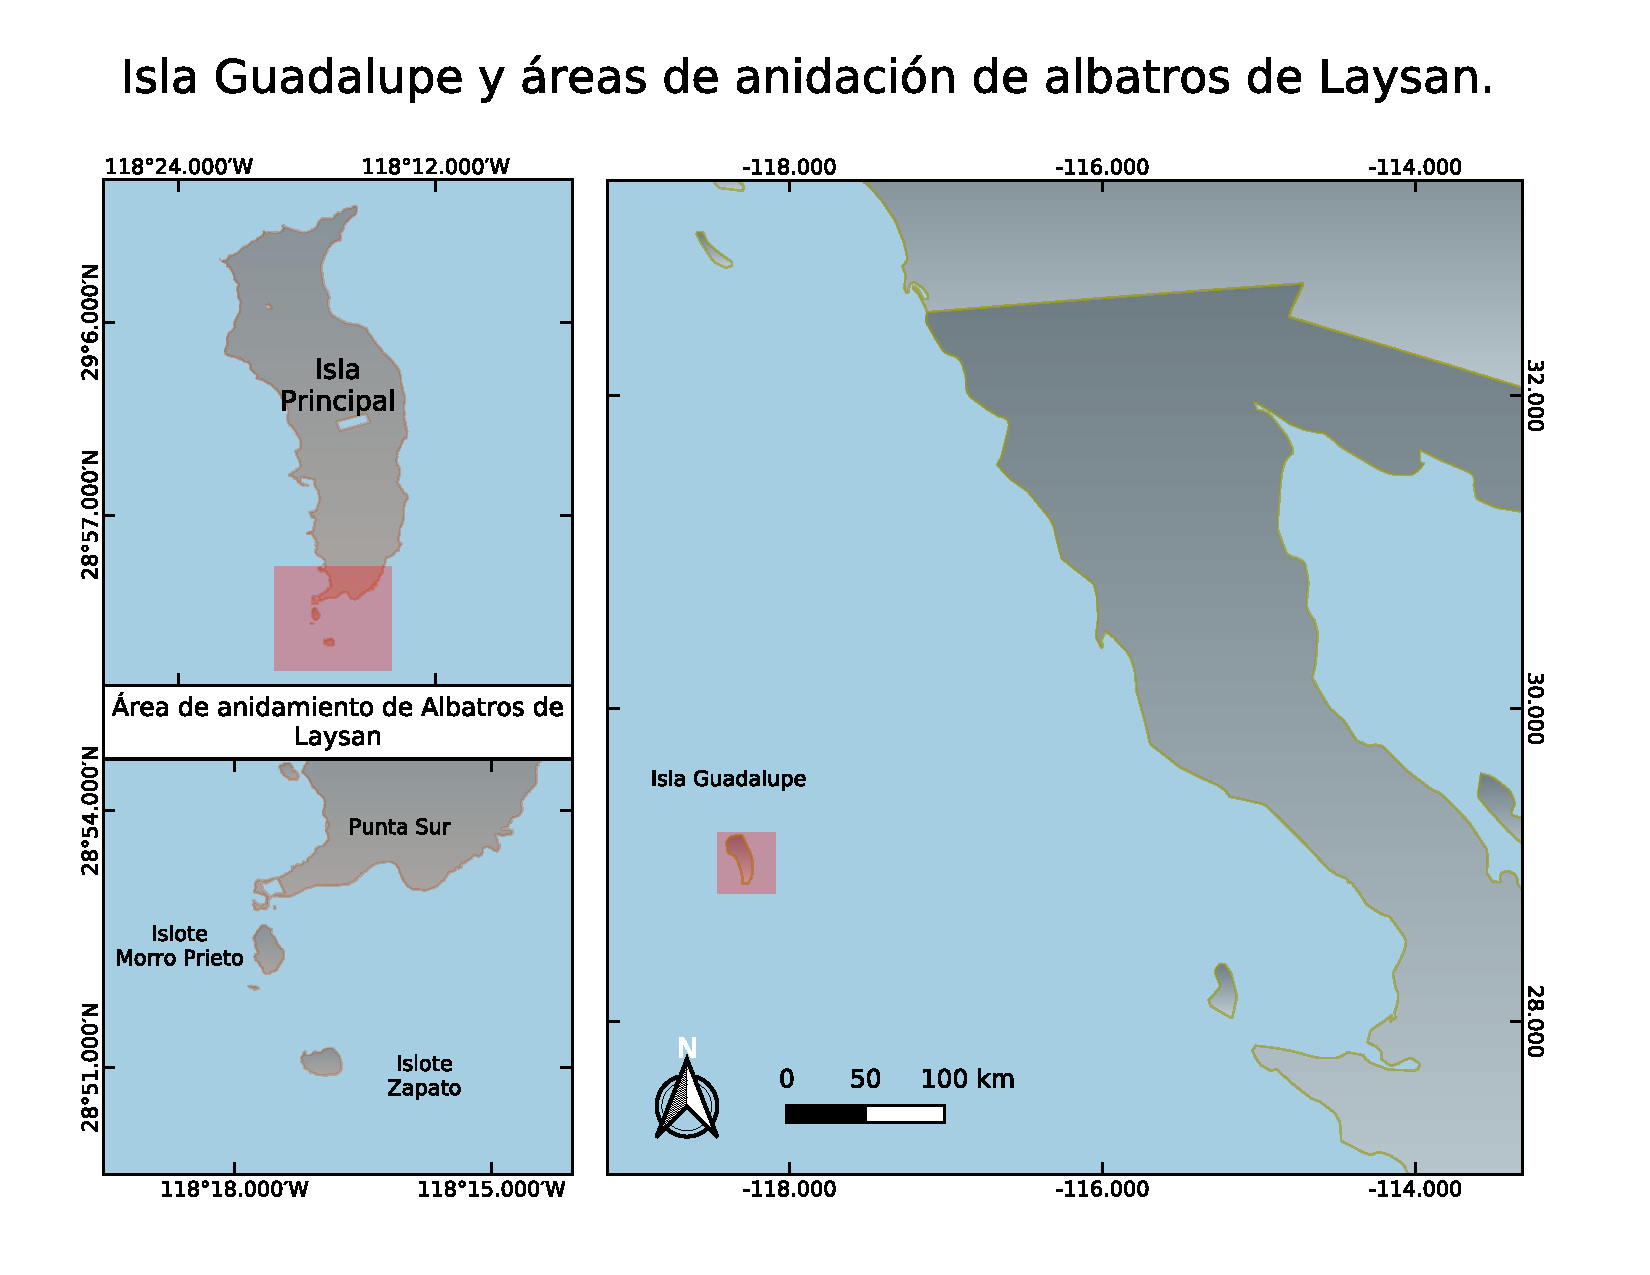
\includegraphics[scale=0.60]{figures/Isla Guadalupe.pdf}
    \caption{Ubicación del área de estudio}
    \label{fig:ubicacionIslaGpe}
    \centering
\end{figure}

\subsection{Creación de base de datos}

\lstinputlisting[language=SQL,   
framesep=10pt, framextopmargin=10pt] {../src/create_table_albatross.sql}

\begin{figure}[h!]
    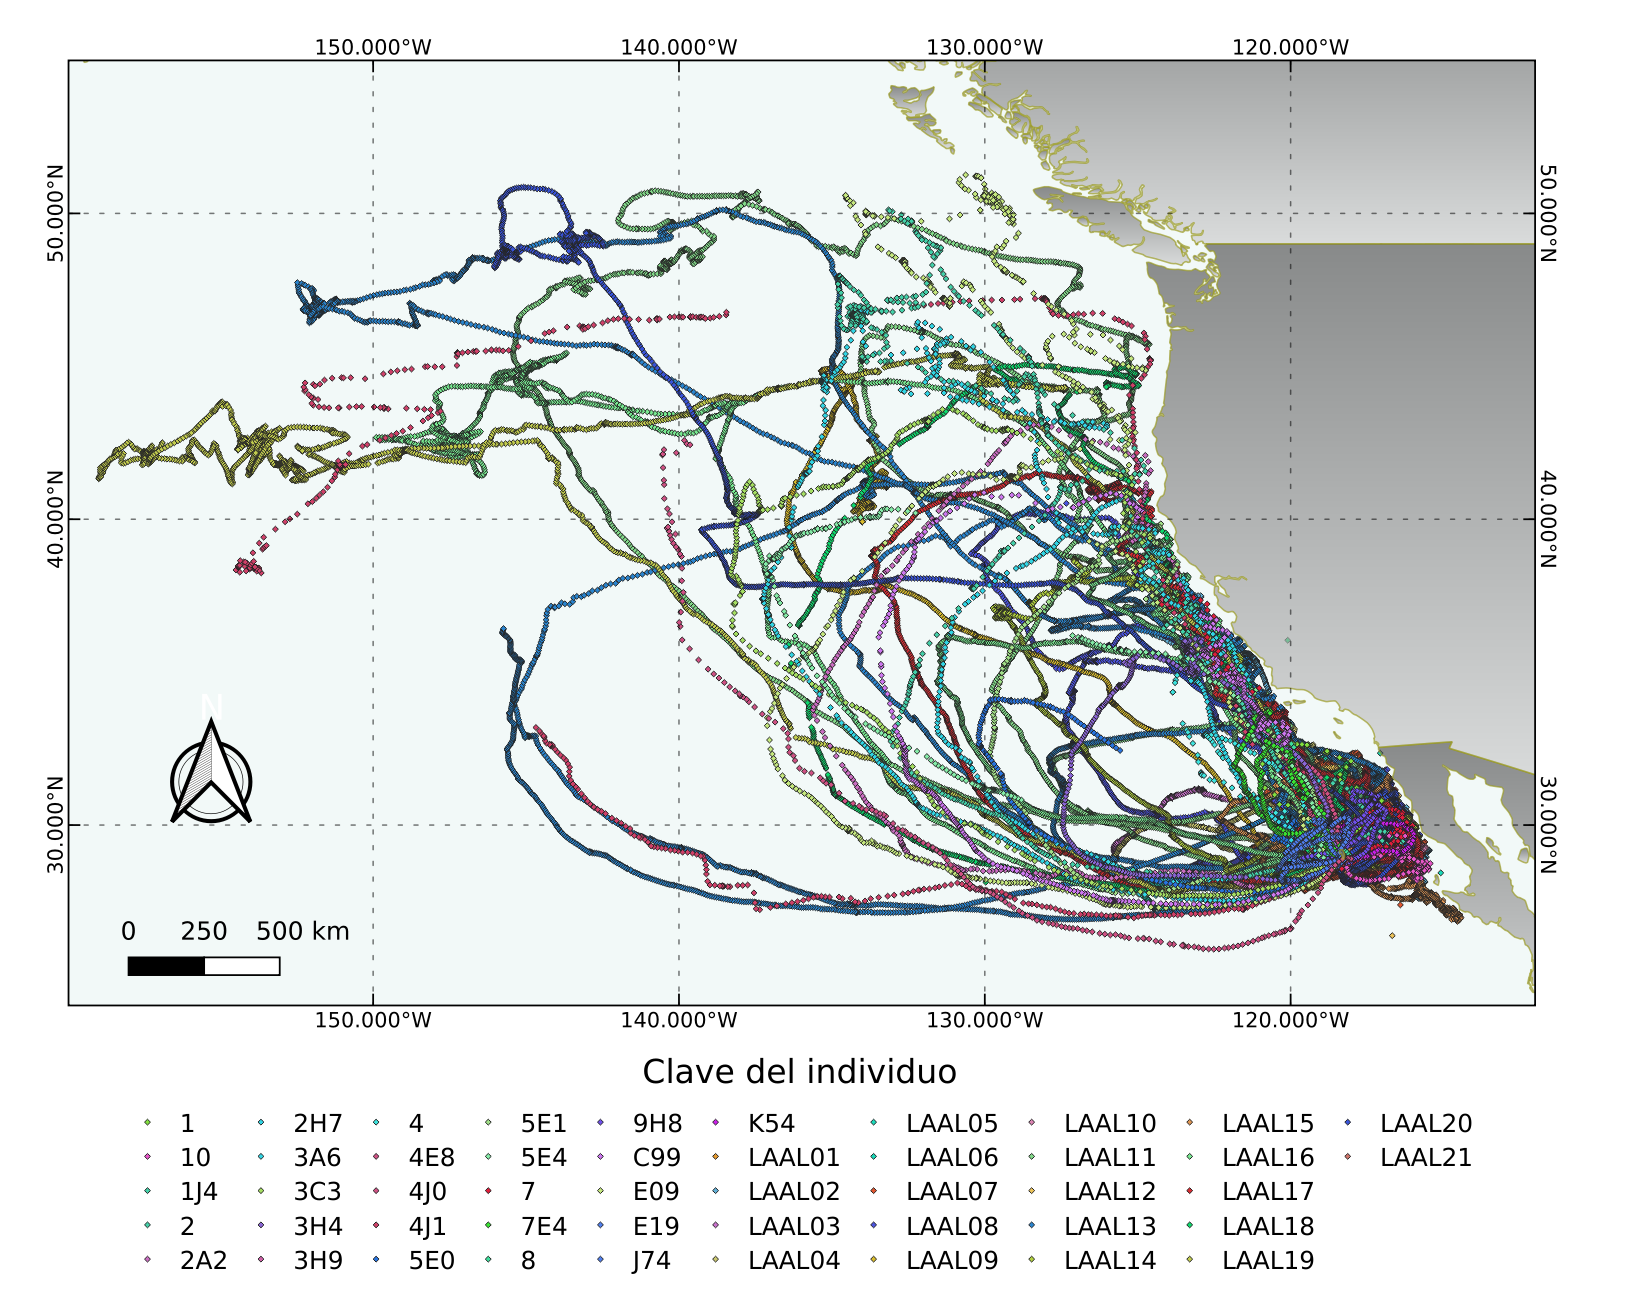
\includegraphics[scale=0.60]{figures/RawData.png}
    \caption{Datos crudos de las trayectorias de albatros}
    \label{fig:trayectorias}
    \centering
\end{figure}
